\section{Finger names}

When playing guitar, your fingers will be given a name. This makes it easier in music notation to indicate which finger should be used. The names are shown in \autoref{fig:finger_names}.

\begin{figure}[h]
    \centering
    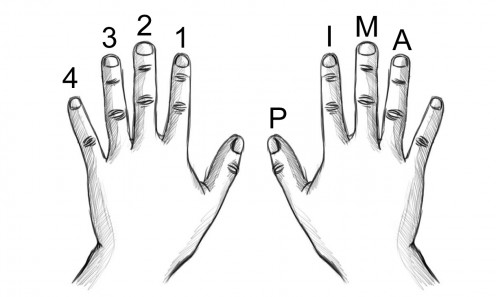
\includegraphics[width=0.7\textwidth]{../../Images/guitar-finger-tips_pima.jpg}
    \caption{Names of the fingers \cite{FingerNames}}
    \label{fig:finger_names}
\end{figure}

\autoref{fig:left_hand_position} shows how to position your left hand. The most important thing is to have your fingertips almost completely perpendicular on the string. This makes sure that you get a clean sound and don't accidentally touch or mute other strings.

Sometimes, however, there is a sequence of notes that would require you to play a single finger over two of more strings. But it general. Keep your fingers perpendicular on the strings.

\begin{figure}[h]
	\begin{subfigure}[b]{0.45\textwidth}
		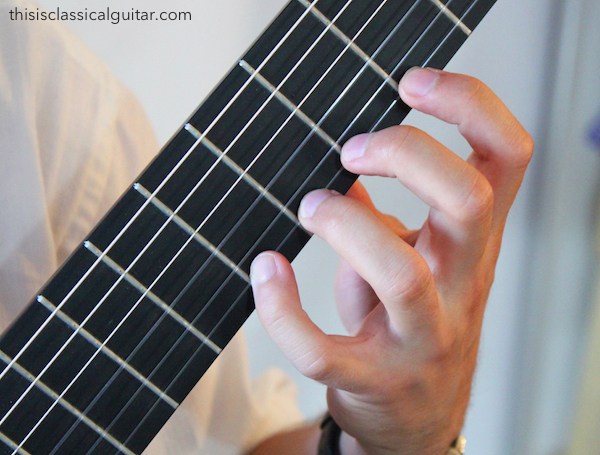
\includegraphics[width=\textwidth]{../../Images/Brad-left-finger-position-front-2016.jpg}
		\caption{}
		\label{fig:}
	\end{subfigure}
	\hfill
	\begin{subfigure}[b]{0.45\textwidth}
		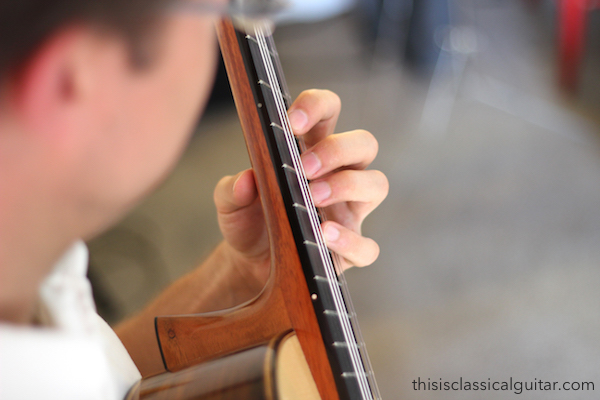
\includegraphics[width=\textwidth]{../../Images/Bradford-Left-hand-player-2016.jpg}
		\caption{}
		\label{fig:}
	\end{subfigure}
	\caption{Left hand position \cite{LeftHandPositionBradlyWerner}}
	\label{fig:left_hand_position}
\end{figure}

\newpage

\section{Free and rest stroke}

With a free stroke you hold your right hand in a relaxed position over the strings (see \autoref{fig:free_stoke_hand_position}). To play a string, move your finger through the string without lifting the upper part of your finger. Your finger should slightly curl into your hand. Once you made the sound, move your finger back to the relaxed position.

The trick now is to not hit the other strings, and to not pluck/pull the string.

\begin{figure}[h]
  \begin{subfigure}[b]{0.45\textwidth}
    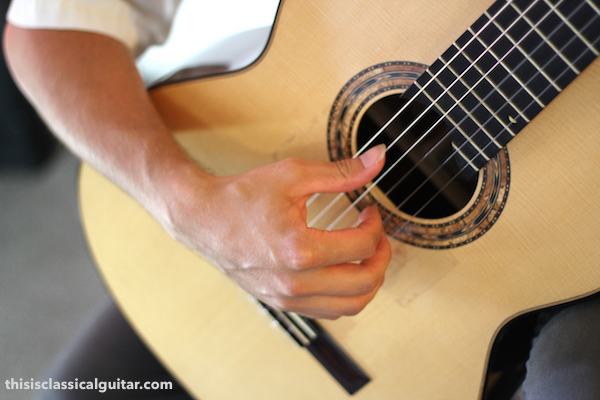
\includegraphics[width=\textwidth]{../../Images/Bradford-right-hand-close-2016.jpg}
    \caption{}
    \label{fig:}
  \end{subfigure}
  \hfill
  \begin{subfigure}[b]{0.45\textwidth}
    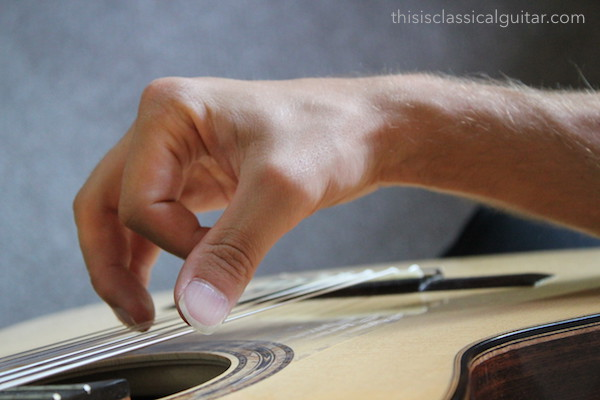
\includegraphics[width=\textwidth]{../../Images/brad-right-stroke-2016.jpg}
    \caption{}
    \label{fig:}
  \end{subfigure}
  \caption{Free stroke position \cite{FreeStrokePositionBradlyWerner}}
  \label{fig:free_stoke_hand_position}
\end{figure}

A rest stroke may sound a bit louder (but with some practicing a free stroke can be as loud). Like the name suggests, a rest stroke means that you move your finger through a string to play it, but now you let your finger rest on the next string.

\section{Using a pick}

Besides fingers, you can also play guitar with a pick (also called a plectrum).

While there is no single correct way to hold a pick, \autoref{fig:how_to_hold_a_pick} is a good starting point. The most important thing is that you don't grip too loose or too strong on the pick. Also, try to not bend you thumb inwards, but a either keep it straight or a little bit bend outwards.

To pick smooth through the string. Don't place the pick flat on the string. Instead, keep the pick at a small angle so that the string slides a little bit over the edge of the pick. Just a small angle is sufficient.

\begin{figure}[h]
	\begin{subfigure}[b]{0.45\textwidth}
		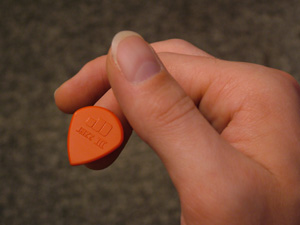
\includegraphics[width=\textwidth]{../../Images/JustinGuitarPickhold1.jpg}
		\caption{}
		\label{fig:}
	\end{subfigure}
	\hfill
	\begin{subfigure}[b]{0.45\textwidth}
		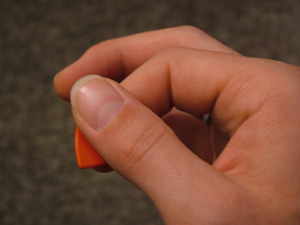
\includegraphics[width=\textwidth]{../../Images/JustinGuitarPickhold2.jpg}
		\caption{}
		\label{fig:}
	\end{subfigure}
	\caption{How to hold a pick \cite{JustinGuitarPickHolding}}
	\label{fig:how_to_hold_a_pick}
\end{figure}

\newpage

\section{Exercises}

In the exercises below you see some symbols above the notes. The numbers with circles around them indicate on which string the note should be played. The \textit{i} and \textit{m} indicate which right-hand finger should be used to play the note.

Try playing \autoref{fig:exercise_rest_free_stroke} with a free stroke, rest stroke, and a pick to hear the differences. If you play with a pick, the \textit{i} and \textit{m} indication of course can be ignored.

When playing with a pick, try to play once with only downstrokes, and once with alternate picking. Downstrokes mean that you only play notes by placing the pick on a string, and then push through and place the pick back on the string again. Alternate picking starts the same as a single downpick. But instead of going on top of the string again after the first note, you play the note by pushing the pick upwards through the string. Then you start with a downpick again and continue alternating.

\begin{figure}[h]
    \centering
    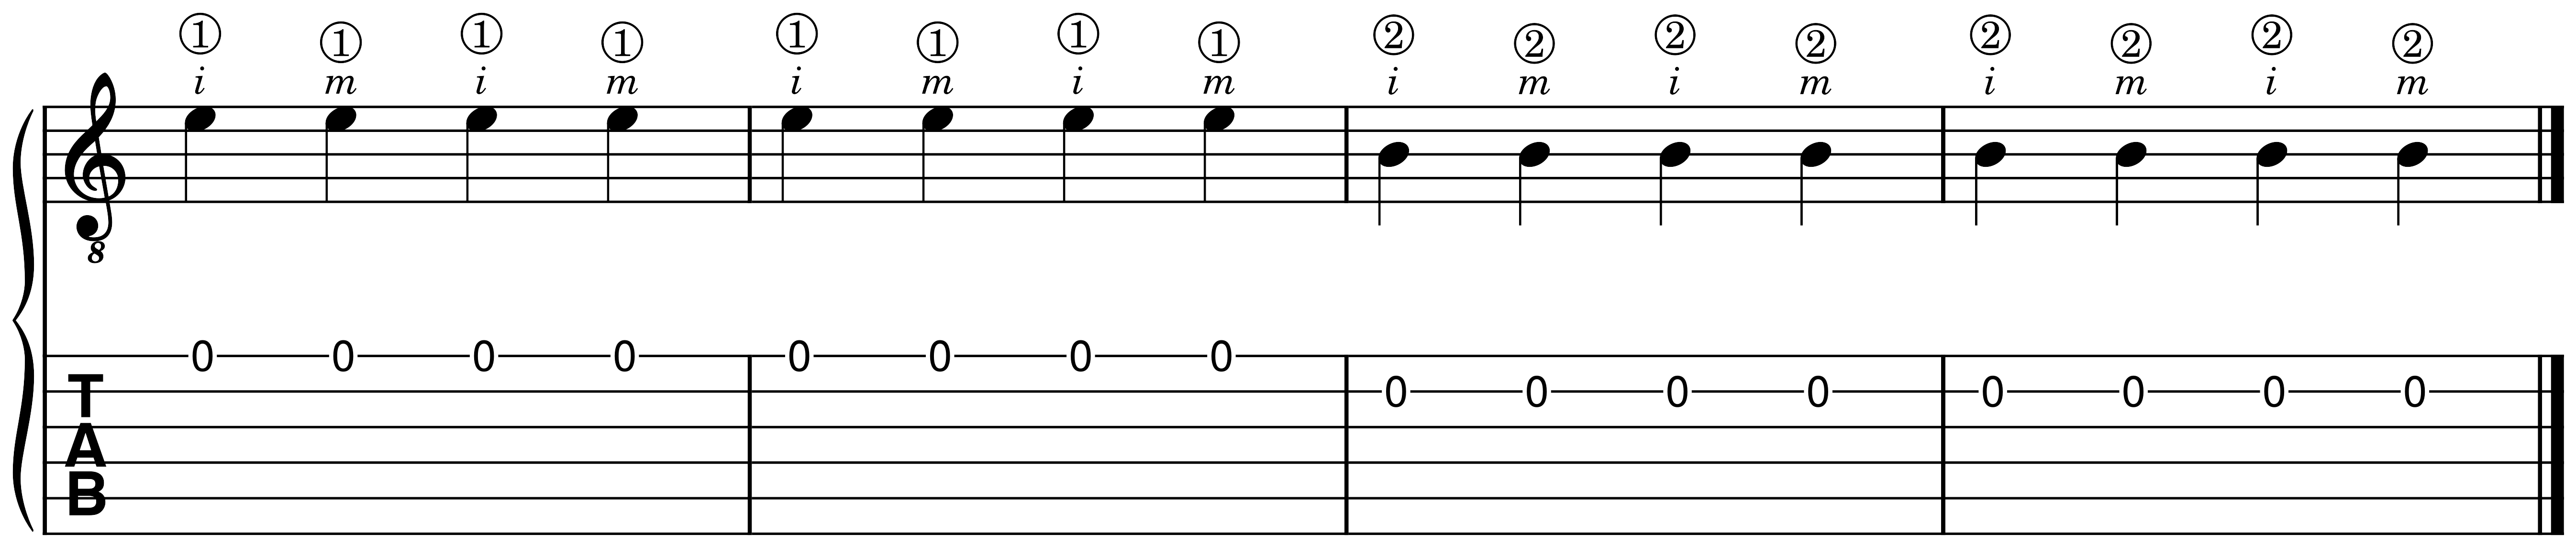
\includegraphics[width=\textwidth]{../../MuseScore/Guitar/OpenEnVallendeAanslag.png}
    \caption{Exercise: rest and free strokes}
    \label{fig:exercise_rest_free_stroke}
\end{figure}

This second exercise (\autoref{fig:exercise_i_m_string_change}) is similar to \autoref{fig:exercise_rest_free_stroke}, but a bit more challenging.

\begin{figure}[h]
    \centering
    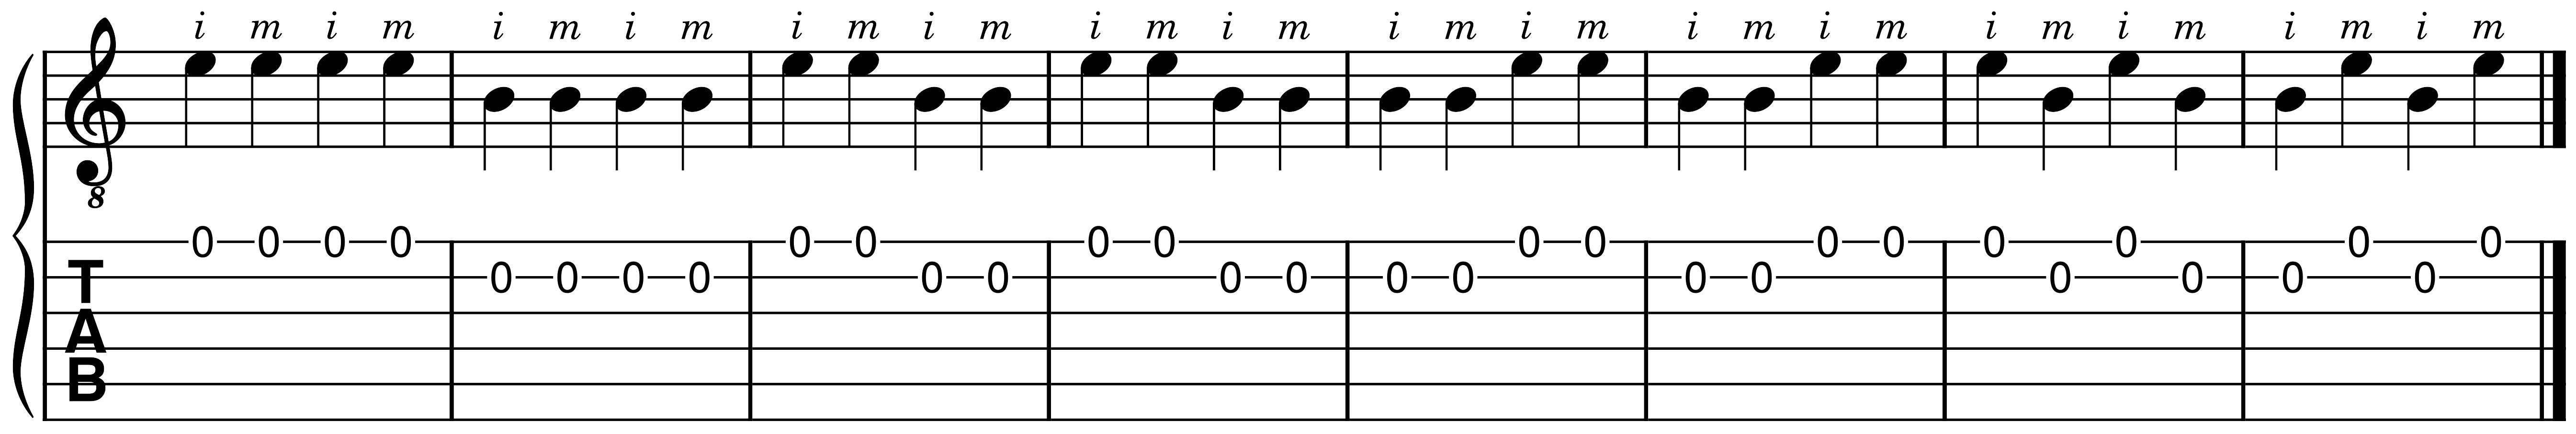
\includegraphics[width=\textwidth]{../../MuseScore/Guitar/TwoStringAlternating.png}
    \caption{Exercise: changing strings with \textit{i} and \textit{m} fingers}
    \label{fig:exercise_i_m_string_change}
\end{figure}

To make use of all PIMA fingers, try to play the intro of \textit{Nothing Else Matters} from \textit{Metallica} (\autoref{fig:exercise_nothing_else_matters_metallica_intro_pima}). You can also try to play this with a pick.

\begin{figure}[h]
    \centering
    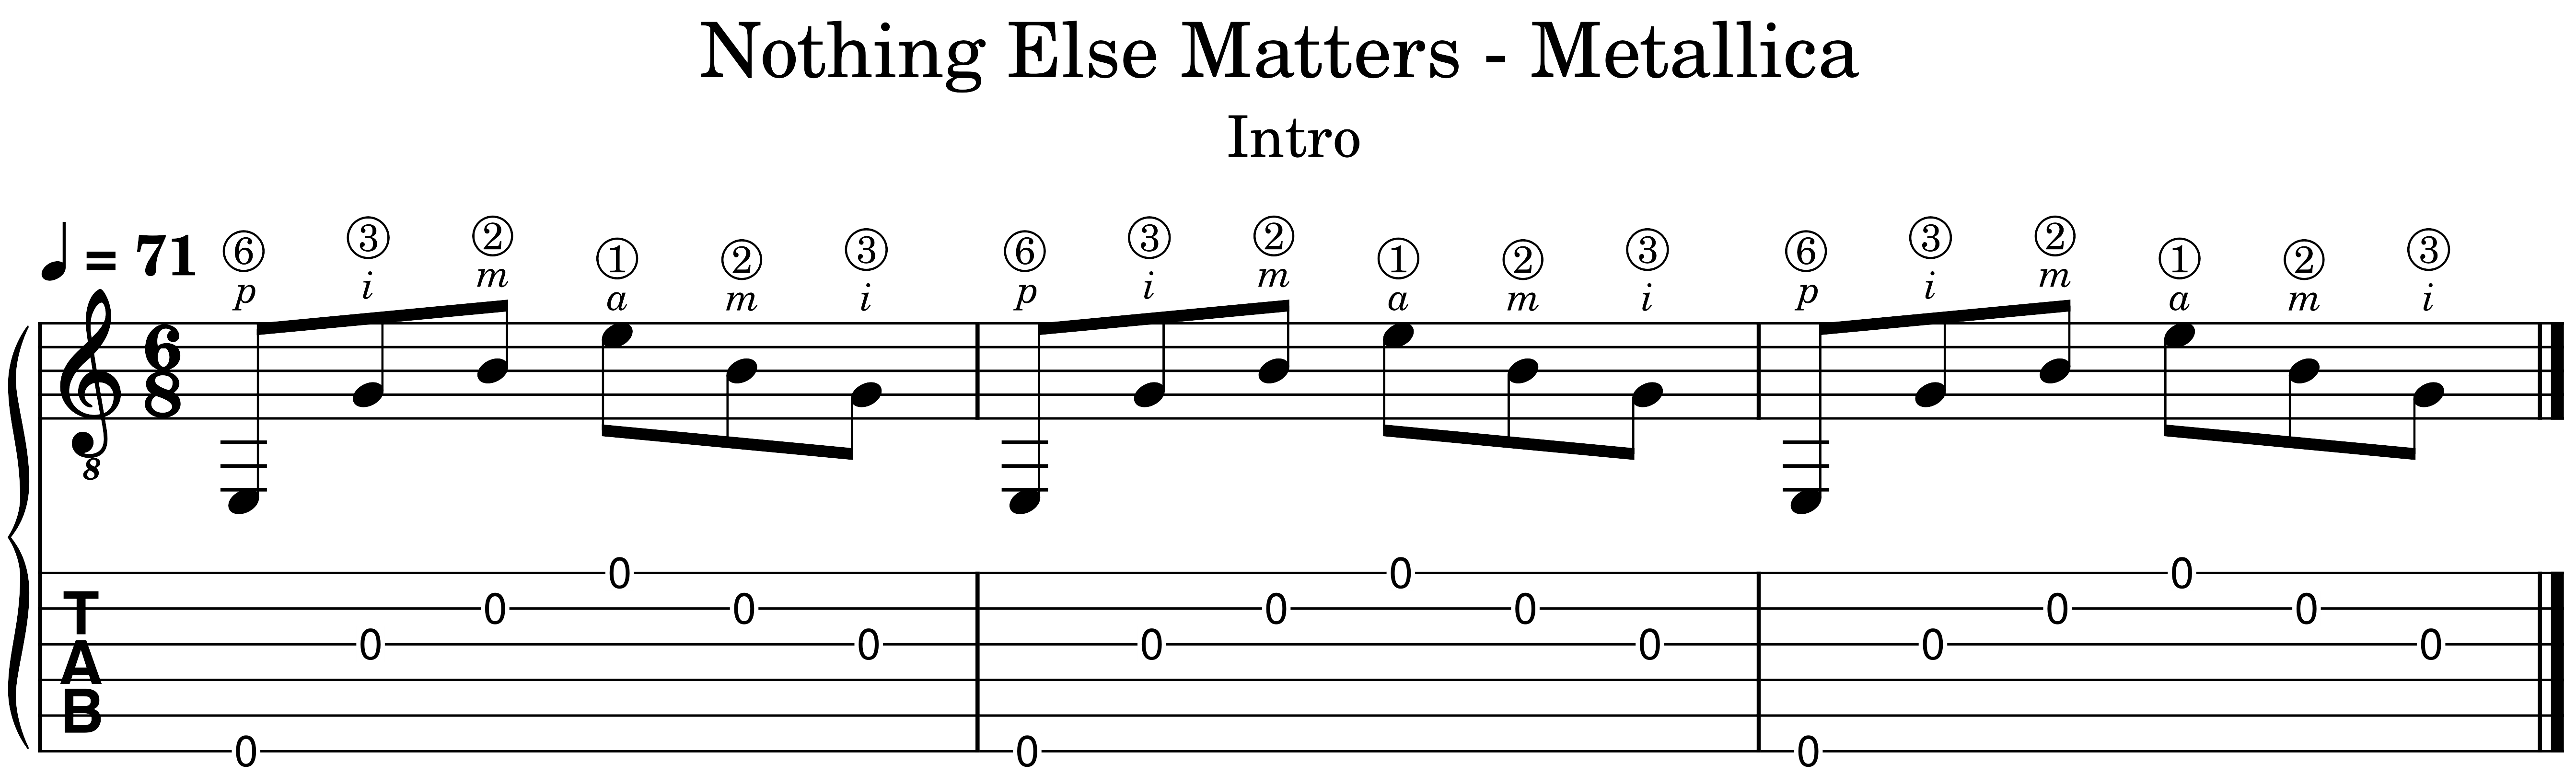
\includegraphics[width=\textwidth]{../../MuseScore/Guitar/NothinElseMatters_Metallica_Intro.png}
    \caption{Exercise: PIMA with Nothing Else Matters - Metallica intro}
    \label{fig:exercise_nothing_else_matters_metallica_intro_pima}
\end{figure}

\newpage

In \autoref{fig:guitar_finger_exercise_perfect_ed_sheeran} you will also use your left hand. The numbers above the notes indicate which left-hand finger should be used to press the fret. Play this exercise using alternating \textit{i} and \textit{m} fingers. Again, you can also use a pick.

Focus on the tabs for now and ignore the other symbols.

\begin{figure}[h]
    \centering
    
\includegraphics[width=\textwidth]{../../MuseScore/Guitar/GuitarPerfectEdSheeranSingleNotesFirstVerse.png}
    \caption{Finger exercise using Perfect - Ed Sheeran}
    \label{fig:guitar_finger_exercise_perfect_ed_sheeran}
\end{figure}